\RequirePackage{plautopatch}
\RequirePackage[l2tabu, orthodox]{nag}

\documentclass[platex,dvipdfmx, titlepage]{jlreq}			% for platex
% \documentclass[uplatex,dvipdfmx]{jlreq}		% for uplatex
\usepackage{graphicx}
\usepackage{bxtexlogo}
\usepackage{braket} % ブラケット
\usepackage{amsmath} % 行列
\usepackage{comment} % コメント
\usepackage{url} % URL
\usepackage{tikz}
\usepackage{physics}
% \usepackage{qcircuit} % 量子回路
\usepackage{array}
\usepackage{quantikz}

\title{初期状態が不完全なグローバーのアルゴリズムの振る舞いについて}

\author{9BSP1118 村岡海人}
\date{\today}
\begin{document}
\maketitle
\tableofcontents
\clearpage

\makeatletter
\renewcommand{\theequation}{%
\thesection.\arabic{equation}}
\@addtoreset{equation}{section}
\makeatother

\section{はじめに}
\begin{comment}
    はじめに
\end{comment}

% \subsection{研究の背景}
% 量子コンピュータとは、量子力学を利用して計算を行うコンピュータである。
% % 量子コンピュータについてもっと詳しく書く
% この量子コンピュータで行う計算を量子計算と呼び、量子計算におけるアルゴリズムのことを量子アルゴリズムと呼ぶ。
% 例えば、多項式時間で整数を因数分解するショアのアルゴリズムや、整列化されていないデータベースからデータベースから特定のデータを探索するグローバーのアルゴリズムがある。


% \subsection{研究の目的}
% 従来の計算機が論理演算から構成されているのと同様、量子計算も量子演算から構成されており、この量子演算は、時間に依存するシュレディンガー方程式から記述することができる。
% 量子計算を行う際に、ハミルトニアンや時間がズレてしまうと実現したい操作からズレた操作を行うことになり、アルゴリズム自体の出力に対す るエラーになってしまう。
% 本研究では、初期状態を準備する操作が不完全な場合に、グローバーのアルゴリズムがどれだけ機能するか調べることを目的とした。
% \subsection{本論文の構成}
% % 大部分が書き終えてから

\section{基本的内容}
\begin{comment}
    基本的内容
\end{comment}


\subsection{量子ビット}
ビットは古典計算と古典情報の基本概念である。
量子計算と量子情報は類似の概念である量子ビットの上に構築される。
\subsubsection{単一量子ビット}
% \input /singleQubit.tex
% 単一量子ビット

まず、量子ビットの説明をする。
古典ビットに1あるいは0の状態に対応した、
状態$\ket{0} = \begin{pmatrix}
    1 \\
    0
\end{pmatrix}$と$\ket{1} = \begin{pmatrix}
    0 \\
    1
\end{pmatrix}$がある。
ここで、量子状態を表すために、ケット記号($\ket{}$)を使ったディラックの記法を用意した。
量子ビットと古典ビットの違いは、量子ビットは$\ket{0}$と$\ket{1}$の重ね合わせ状態を取り得ることである。
これは次のように$\ket{0}$と$\ket{1}$の線型結合として、

\begin{equation}
    \label{eq: QuantumComputationAndQuantumInfomation.1.1}
    \ket{\psi} = \alpha \ket{0} + \beta \ket{1}
\end{equation}

と表される。ここで、$\alpha, \beta$は複素数であり、複素確率振幅と呼ぶ。
量子ビットの状態は2次元複素ベクトル空間のベクトルで表される。
特に$\ket{0}$と$\ket{1}$計算基底状態と呼び、この2次元複素ベクトル空間の正規直交基底を構成する。

古典計算では、古典ビットを調べてそれが0, 1のいずれの状態にあるかを決めることができる。
例えば、コンピュータがメモリの内容を取り出す時にいつもこれを行なっている。
量子ビットは量子ビットを調べてその量子状態、つまり、$\alpha$と$\beta$の値を決めることはできない。
量子ビットに対して$\ket{0}$と$\ket{1}$のいずれの状態にあるかを調べる測定を行うと、確率$|\alpha|^2$で$\ket{0}$、確率$|\beta|^2$で$\ket{1}$が得られる。
全確率の和は$1$なので、$|\alpha|^2 + |\beta|^2 = 1$である。
幾何学的解釈ではこれは量子ビットの状態が長さ1に正規化される条件である。
したがって、一般的に量子ビットの状態は2次元複素ベクトル空間の単位ベクトルを表す。

% TODO: ここはもう少し具体的に修正
量子ビットは自由度が2の多くの系で実現されている。
例えば、核スピン、単一光子の2つの異なる偏光、単一原子における電子軌道の2つの状態などがある。
原子モデルで電子は基底状態、または励起状態に存在しそれぞれを$\ket{0}, \ket{1}$と呼ぶ。

% ブロッホ球のことについて
次のような幾何学的表現が量子ビットを考える上で有用な描像である。
$|\alpha|^2 + |\beta|^2 = 1$であるので、式(\ref{eq: QuantumComputationAndQuantumInfomation.1.1})を次のように書き換える。

% \begin{equation}
%     \label{eq: QuantumComputationAndQuantumInfomation.1.3}
%     \ket{\psi} = e^{i \gamma} \left( \cos{\frac{\theta}{2}} \ket{0} + e^{i\varphi} \sin{\frac{\theta}{2}} \ket{1} \right)
% \end{equation}
% ここで、$\theta, \varphi, \gamma$は実数である。

\begin{equation}
    \label{eq: QuantumComputationAndQuantumInfomation.1.4}
    \ket{\psi} = \cos{\frac{\theta}{2}} \ket{0} + e^{i \varphi} \sin{\frac{\theta}{2}} \ket{1}
\end{equation}
ここで、$\theta, \varphi$は実数である。
図に示すように、$\theta, \varphi$は3次元単位球面上の点を定義する。
この球面をブロッホ球と呼ぶ。

% ブロッホ球の図
\begin{figure}[htbp]
    \label{fig: bloch球}
    \centering
    \tikz{
  \tikzstyle{st}=[lightgray, fill, fill opacity=0.1]
  \coordinate(o)at(0,0);
  \draw(o)circle(2cm);
  \draw[fill](o)circle(1.5pt);%origin
  \draw[st](o)--(56.7:0.4)arc(56.7:90.:0.4)--cycle;%theta angle
  \draw(0.18,0.6)node{$\theta$};
  \draw[st](o)--(-135.7:0.4)arc(-135.7:-33.2:0.4)--cycle;%varphi angle
  \draw(0.14,-0.58)node{$\varphi$};
  \draw[->](o)--(-0.81,-0.79) node[above left]{$x$};%x
  \draw[->](o)--(2,0)node[right]{$y$};%y
  \draw[->](o)--(0,2)node[below right]{$z$}node[above]{$\ket{0}$};%z |0>
  \draw[rotate around={0.:(0.,0.)},dashed](0,0)ellipse(2cm and 0.9cm);%ellipse
  \draw[thick,->](o)--(0.70,1.07)node[above]{$\ket{\psi}$};%state vector
  \draw[densely dotted,->](o)--(0,-2)node[below]{$\ket{1}$};%-z |1>
  \draw[dotted](o)--(0.7,-0.46)--(0.7,1);%triangle
}
\caption{量子ビットのブロッホ球表示}
\end{figure}

これは単一量子ビット状態を視覚化する便利な方法である。
単一量子ビットの操作はブロッホ球上の描像で記述できる。
しかし、ブロッホ球は多量子ビットに対して一般化できないことに注意する。

\subsubsection{多量子ビット}
% \input 基本的内容/multipleQubit.tex
\begin{comment}
    多量子ビット
\end{comment}


多量子ビットの状態について考えてみる。
簡単のため、2個の量子ビットがあるとする。
これが古典ビットならば4つの取り得る状態$00, 01, 10, 11$がある。
これに対して2個の量子ビットの系には$\ket{00}, \ket{01}, \ket{10} \ket{11}$で表される計算基底状態がある。
2個の量子ビットを記述する状態ベクトルは、
\begin{equation}
    \label{eq: QuantumComputationAndQuantumInfomation.1.5}
    \ket{\psi} = \alpha_{00} \ket{00} + \alpha_{01} \ket{01} + \alpha_{10} \ket{10} + \alpha_{11} \ket{11}
\end{equation}
で与えられる。
ここで、$\alpha_{00}, \alpha_{01}, \alpha_{10}, \alpha_{11}$はそれぞれの基底の複素確率振幅である。
単一量子ビットの場合と同様に、測定結果$x(= 00, 01, 10, 11)$は確率$|\alpha_x|^2$で生じ、測定後の量子ビットの状態は$\ket{x}$となる。
確率の合計が1になる条件は正規化状態$\sum_{x \in \{0, 1\}^2} |\alpha_x|^2 = 1$で表される。
ここで、記号「$\{0, 1\}^2$」は「各文字が0または1であり、長さ2の記号列の集合」を意味する。

一般に$n$個の量子ビットを考えると、この系の計算基底は$\ket{x_1 x_2 \cdots x_n}$の形をしており、この系の量子状態は$2^n$個の振幅で規定される。
ここで、$x = x_1 x_2 \cdots x_3$は、$x \in \{ 0, 1 \}^n$であり、$x \in \{ 0, 1 \}^n$は各文字が$0$または$1$であり、長さ$n$の記号列の集合を表す。

\subsection{量子計算}
% \input 基本的内容/quantumComputing.tex
\begin{comment}
    多量子ビット
\end{comment}


多量子ビットの状態について考えてみる。
簡単のため、2個の量子ビットがあるとする。
これが古典ビットならば4つの取り得る状態$00, 01, 10, 11$がある。
これに対して2個の量子ビットの系には$\ket{00}, \ket{01}, \ket{10} \ket{11}$で表される計算基底状態がある。
2個の量子ビットを記述する状態ベクトルは、
\begin{equation}
    \label{eq: QuantumComputationAndQuantumInfomation.1.5}
    \ket{\psi} = \alpha_{00} \ket{00} + \alpha_{01} \ket{01} + \alpha_{10} \ket{10} + \alpha_{11} \ket{11}
\end{equation}
で与えられる。
ここで、$\alpha_{00}, \alpha_{01}, \alpha_{10}, \alpha_{11}$はそれぞれの基底の複素確率振幅である。
単一量子ビットの場合と同様に、測定結果$x(= 00, 01, 10, 11)$は確率$|\alpha_x|^2$で生じ、測定後の量子ビットの状態は$\ket{x}$となる。
確率の合計が1になる条件は正規化状態$\sum_{x \in \{0, 1\}^2} |\alpha_x|^2 = 1$で表される。
ここで、記号「$\{0, 1\}^2$」は「各文字が0または1であり、長さ2の記号列の集合」を意味する。

一般に$n$個の量子ビットを考えると、この系の計算基底は$\ket{x_1 x_2 \cdots x_n}$の形をしており、この系の量子状態は$2^n$個の振幅で規定される。
ここで、$x = x_1 x_2 \cdots x_3$は、$x \in \{ 0, 1 \}^n$であり、$x \in \{ 0, 1 \}^n$は各文字が$0$または$1$であり、長さ$n$の記号列の集合を表す。

\subsection{量子アルゴリズムと量子並列性}
\begin{comment}
    量子アルゴリズムについての記述
    24
\end{comment}

量子コンピュータは、量子力学的な重ね合わせによって、$n$個の量子ビットを用いて$2^n$個の状態を同時に処理できる。
しかし、これだけでは「計算が速い」ということにはならない。
なぜなら、計算終了後に結果を観測する際に、$2^n$個の状態の内どれか1つがランダムに得られるのみだからである。
したがって、欲しい答えが高確率で得られるように設計された、量子コンピュータ専用のアルゴリズムが不可欠である。
そのようなアルゴリズムを量子アルゴリズムと呼ぶ\cite{QuantumDojo}。


% 量子アルゴリズムの有名な例として、Shorの量子フーリエ変換と、本研究の対象であるグローバーのアルゴリズムがある。
% Shorの量子フーリエ変換は素因数分解や離散対数問題を解くアルゴリズムに基づいている。
% 最良の古典アルゴリズムに比べて指数関数的な著しい高速化を実現する。
% グローバーのアルゴリズムは

量子アルゴリズムのクラスは主に2つ存在する。
最初のクラスは素因数分解や離散対数問題を解くアルゴリズムを含む、Shorの量子フーリエ変換に基づくものであり、最良の古典アルゴリズムに比べて指数関数的な著しい高速化を実現する。
2つ目のアルゴリズムのクラスは量子探索を行うグローバーのアルゴリズムに基づくものである。
これはそれほど著しくないが、それでも最良の古典アルゴリズムに比べて、2乗の顕著な高速化を実現する。
量子探索アルゴリズムはが重要なのは古典アルゴリズムで探索ベースの技術が広く使われており、多くの事例で古典アルゴリズムを高速の量子アルゴリズムに直接変更することができるからである\cite{QuantumComputation&Infomation2}。

\subsection{グローバーのアルゴリズム}
\begin{comment}
    ここではグローバーのアルゴリズムについて記述する
\end{comment}

\subsection{グローバーのアルゴリズム}
本節では、データベース探索など、いわゆる探索問題を解く量子アルゴリズムを説明する。
量子探索アルゴリズムは古典の探索アルゴリズムより計算量が少なく、高速であると言われている。
% ここでいう計算量とはオラクルという関数にアクセスする回数で定義されている。

\subsubsection{概要}
このグローバーのアルゴリズムは以下のような流れで行う。
$N$個のデータに対して$O(\sqrt{N})$回の計算量で解を見出すことができる。
古典的な探索アルゴリズムでも同じ計算量を持つ2分探索アルゴリズムがあるが、2分探索アルゴリズムは事前にソートされているデータを扱うため、
ソートされていないデータの探索アルゴリズムではグローバーのアルゴリズムの方が高速である。

このグローバーのアルゴリズムは以下のような流れで行う。
$n$を量子ビット数とすると、$N = 2^n$の要素からなるデータベースから$M$個の解を探索する問題を考え、要素のラベルを$n$桁のビット列$x = x_1 \cdots x_n$とする。

\begin{itemize}
    \item 全ての状態の重ね合わせ状態$\ket{s} = \frac{1}{N} \sum_{x} \ket{x}$を用意する
    \item 演算子$U_w$(解に対する反転操作)を作用させる
    \item 演算子$U_s$($\ket{s}$を対象軸にした反転操作)を作用させる
    \item 2、3を$k$回繰り返す
\end{itemize}

\subsubsection{アルゴリズムの流れ}
まず初めに、全ての状態の重ね合わせ状態$\ket{s} = \frac{1}{\sqrt{N}} \sum_{x} \ket{x}$を用意する。
初期状態$\ket{0}^{\otimes n} = \ket{0 \cdots 0}$に対して全ての量子ビットにアダマール演算子を作用させると、

\begin{equation}
    \begin{split}
      \ket{s} &= H^{\otimes n}\ket{0}^{\otimes n} \\
      &= (H \otimes \cdots \otimes H)\ket{0 \cdots 0} \\
      &= \frac{1}{\sqrt{2^n}}(\ket{0} + \ket{1}) \otimes \cdots \otimes (\ket{0} + \ket{1}) \\
      \ket{s} &= \frac{1}{\sqrt{2^n}} \sum_{x = 0}^{2^n - 1}
    \end{split}
\end{equation}
のように計算できる。

次に解に対する反転操作を作用させる。
入力$\ket{x}$に対して$x$が解なら、$-1$をかけて位相を反転し、解でないならば1をかける。
つまり、単一量子ゲートを以下のように定義する。
\begin{equation}
    \left\{ 
    \begin{alignedat}{2}   
        U_w \ket{x} &= \ket{x} \ (x \ne w) \\
        U_w \ket{w} &= - \ket{w}
    \end{alignedat} 
    \right.
\end{equation}

\begin{equation}
    U_w = I - 2 \sum_{w \in 解} \ket{w}\bra{w}
\end{equation}
$w$は検索したい値である。
これを用いいると、$\ket{s}$は、
\begin{equation}
    \label{eq:Uws}
    \begin{split}
        U_w &= \frac{1}{\sqrt{2^n}} \sum_{x = 0, x \ne w}^{2^n - 1} U_w \ket{x} + \frac{1}{\sqrt{2^n}}U_w \ket{x} \\
        &= \frac{1}{\sqrt{2^n}} \sum_{x = 0, x \ne w}^{2^n - 1} \ket{x} - \frac{1}{\sqrt{2^n}} \ket{w} \\
        U_w \ket{s} &= \ket{s} - \frac{2}{\sqrt{2^n}} \ket{w}
    \end{split}
\end{equation}
のように計算できる。

最後に、$\ket{s}$を対象軸にした反転操作$U_s$を定義する。

\begin{equation}
    \left\{ 
    \begin{alignedat}{2}   
        U_s \ket{x} = 2\bra{s} x \ket{s} - \ket{x} = \frac{2}{\sqrt{2^n}} \ket{x} \\
        U_s \ket{s} = 2 \bra{s} s \ket{s} - \ket{s} = \ket{s}
    \end{alignedat} 
    \right.
\end{equation}

\begin{equation}
    U_s = 2\ket{s}\bra{s} - I
\end{equation}

式(\ref{eq: Uws})より、$U_s$を作用させると、

% \begin{equation}
%     U_s U_w \ket{s} = \ket{s} - \frac{2}{\sqrt{2}}
% \end{equation}

\begin{equation}
    \label{eq:UsUws}
    \begin{split}
        U_s U_w \ket{s} &= \ket{s} - \frac{2}{\sqrt{2}} \left( \frac{2}{\sqrt{2^n}} \ket{s} - \ket{w} \right)\\
        &= \frac{2^n - 4}{2^n} \ket{s} + \frac{2}{\sqrt{2^n}} \ket{w}\\
        &= \frac{2^n - 4}{2^n \sqrt{2^n}} \sum_{x = 0, x \ne w}^{2^n - 1} \ket{x} + \left( \frac{2^n - 4}{2^n \sqrt{2^n}} + \frac{2}{\sqrt{2^n}} \right) \ket{w}\\
        U_s U_w \ket{s} &= \frac{2^n - 4}{2^n \sqrt{2^n}} \sum_{x = 0, x \ne w}^{2^n - 1} \ket{x} + \frac{3 \cdot 2^n - 4}{2^n \sqrt{2^n}} \ket{w}
    \end{split}
\end{equation}

のように計算できる。

$\ket{s}$の時の状態では、$\ket{w}$を測定すると、確率は$\frac{1}{2^n}$となる。
式(\ref{eq: UsUws})から確率が上昇していることがわかる。
この確率を増幅させる操作のことを、反復増幅と呼ぶ。
グローバーのアルゴリズムは、この反復増幅を複数かい行うことにより、$\ket{w}$の確率を1に近づける。


\subsubsection{図を使用しての説明}

$\ket{w}$に直行するベクトル$\ket{w^{\perp}}$を用いた平面を考えると、以下のような状態が得られる。
\begin{equation}
    \ket{w} = \frac{1}{\sqrt{N - M}} \sum^{2^n - 1}_{x = 0, w \neq 0} \ket{x}
\end{equation}

\begin{equation}
    \ket{w^{\perp}} = \frac{1}{\sqrt{M}} \ket{w}
\end{equation}
全ての状態の重ね合せ状態$\ket{s}$は次のように表すことができるので、2次元平面ベクトルであることがわかる。
\begin{equation}
    \label{eq:hgoe}
    \ket{s} = \sqrt{\frac{N - M}{N}} \ket{w^{\perp}} + \sqrt{\frac{M}{N}}\ket{w}
\end{equation}

全ての状態の重ね合わせ状態$\ket{s}$は次のように表せるので、この2次元平面内ベクトルであることがわかる。
% 式(\ref{eq: 3.1})より、$\cos{\frac{\theta}{2}} = \sqrt{\frac{N - M}{N}}, \sin{\frac{\theta}{2}} = \sqrt{\frac{M}{N}}$を満たす角$\theta$を用いれば、
式(\ref{eq: hoge})より、$\cos{\frac{\theta}{2}} = \sqrt{\frac{N - M}{N}}, \sin{\frac{\theta}{2}} = \sqrt{\frac{M}{N}}$を満たす角$\theta$を用いれば、
と表すことができる。
これを図示すると、図\ref{fig:rootate}のようになる。

\begin{equation}
    \ket{s} = \cos{\frac{\theta}{2}} \ket{w^{\perp}} + \sin{\frac{\theta}{2}} \ket{w}
\end{equation}

\begin{figure}[htbp]
    \centering
    \begin{tikzpicture}
        \draw[->,>=stealth,semithick] (-0.5,0)--(4,0)node[above]{$\ket{w^{\perp}}$}; %x軸
        \draw[->,>=stealth,semithick] (0,-0.5)--(0,3.5)node[right]{$\ket{w}$}; %y軸
        \draw (0,0)node[below left]{O}; %原点
        \draw[->] (0,0)--(3, 1.5)node[right]{$\ket{s}$};
        \draw [-](1,0) arc (0:20:1.4);
        \coordinate (thrta_0) at (1,0) node at (thrta_0) [above right] {$\theta / 2$};
    \end{tikzpicture}
    \caption{全ての状態の重ね合わせ状態$\ket{s}$}
    % \label{fig:rootate}
\end{figure}

\begin{figure}[htbp]
    \centering
    \begin{tikzpicture}
        \draw[->,>=stealth,semithick] (-0.5,0)--(4,0)node[above]{$\ket{w^{\perp}}$}; %x軸
        \draw[->,>=stealth,semithick] (0,-0.5)--(0,3.5)node[right]{$\ket{w}$}; %y軸
        \draw (0,0)node[below left]{O}; %原点
        \draw[->, dotted] (0,0)--(3, 1.5)node[right]{$\ket{s}$};
        \coordinate (thrta_0) at (1,0) node at (thrta_0) [above right] {$\theta / 2$};
        \draw [-](1,0) arc (0:20:1.4);
        
        \draw[->] (0,0)--(3, -1.5)node[right]{$U_w \ket{s}$};
        \coordinate (thrta_1) at (1,0) node at (thrta_0) [below right] {$\theta / 2$};
        \draw [-](1,0) arc (0:-20:1.4);
    \end{tikzpicture}
    \caption{$\ket{s}$に$U_w$を作用}
    \label{rootate2}
\end{figure}
次に、$\ket{s}$に$U_w$をかけることにより、$\ket{w^{\perp}}$を軸に反転すると、図\ref{fig:rootate2}のようになる。

最後に、$U_s$を作用させることにより、$\ket{s}$を軸に$U_w \ket{s}$を反転させると、図3のようになる。

\begin{figure}[htbp]
    \centering
    \label{rootate}
    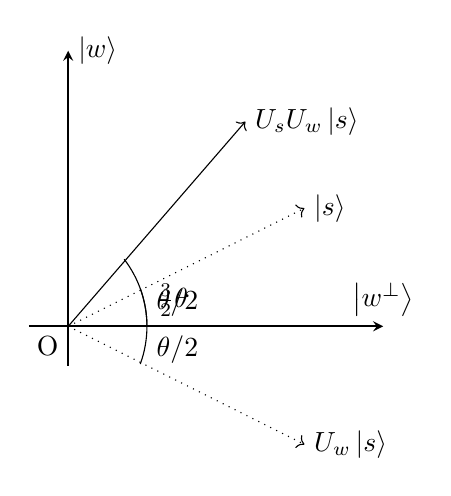
\begin{tikzpicture}
        \draw[->,>=stealth,semithick] (-0.5,0)--(4,0)node[above]{$\ket{w^{\perp}}$}; %x軸
        \draw[->,>=stealth,semithick] (0,-0.5)--(0,3.5)node[right]{$\ket{w}$}; %y軸
        \draw (0,0)node[below left]{O}; %原点
        \draw[->, dotted] (0,0)--(3, 1.5)node[right]{$\ket{s}$};
        \coordinate (thrta_0) at (1,0) node at (thrta_0) [above right] {$\theta / 2$};
        \draw [-](1,0) arc (0:20:1.4);
        
        \draw[->, dotted] (0,0)--(3, -1.5)node[right]{$U_w \ket{s}$};
        \coordinate (thrta_1) at (1,0) node at (thrta_0) [below right] {$\theta / 2$};
        \draw [-](1,0) arc (0:-20:1.4);
        
        \draw[->] (0,0)--(2.25, 2.6)node[right]{$U_s U_w \ket{s}$};
        \coordinate (thrta_0) at (1,0) node at (thrta_1) [above right] {$\frac{3}{2}\theta$};
        \draw [-](1,0) arc (0:37.5:1.4);
    \end{tikzpicture}
    \caption{$U_w\ket{s}$に$U_s$を作用}
\end{figure}

以上より、平面ベクトル内で、角度$\theta$だけの回転が行われ、$\ket{w}$を測定する確率が上昇することがわかる。


% \section{最適な$k$の見積もり}
\subsubsection{最適な$k$の見積もり}
最後に、$U_sU_w$を作用させる回数$k$について、最適な回数が幾つなのか調べる。
式(3.2)より、グローバーのアルゴリズムを1回施すと、
\begin{equation}
    U_sU_w\ket{s} = \cos{\frac{3}{2}\theta}\ket{w^{\perp}} + \sin{\frac{3}{2}\theta}\ket{w}
\end{equation}
となる。これを$k$回施すと、
\begin{equation}
    (U_sU_w)^k\ket{s} = \cos{\frac{2k+1}{2}\theta} \ket{w^{\perp}} + \sin{\frac{2k+1}{2}\theta} \ket{w}
\end{equation}
となる。これを用いて、最終的に$\ket{w}$の確率振幅を1にしたいので、

\begin{equation}
    \begin{split}
        \sin{\frac{2k + 1}{2} \theta} = 1 \\
        \Leftrightarrow \frac{2 k + 1}{2} \theta = \frac{\pi}{2} \\
        k = \frac{\pi}{2 \theta}
    \end{split}
\end{equation}

% \begin{equation}
%     \begin{split}
%             \sin{\frac{2k + 1}{2}\theta} = 1 \\
%             \Leftrightarrow	\frac{2k + 1}{2}\theta = \frac{\pi}{2} \\
%             \therefore k = \frac{\pi}{2 \theta} 
%     \end{split}
% \end{equation}

となる。よって、$\frac{2k + 1}{2}\theta$が$\frac{\pi}{2}$にもっとも近くなるときは、
\begin{equation}
    R = ClosestInteger(\frac{\pi}{2\theta} - \frac{1}{2})
\end{equation}
の時である。ここで、$ClosestInteger(...)$は$...$に最も近い整数を表す。

最後に、Rの上限を評価する。$\theta > 0$について成り立つ式、
\begin{equation}
    \frac{\theta}{2} \geq \sin{\frac{\theta}{2}} = \sqrt{\frac{M}{N}}
\end{equation}
を使うと、以下のように表すことができる。
\begin{equation}
    R \leq \left( \frac{\pi}{2\theta} - \frac{1}{2} \right) + 1 = \frac{\pi}{2\theta} + \frac{1}{2} \leq \frac{\pi}{4}\sqrt{\frac{N}{M}} + \frac{1}{2}
\end{equation}
つまり、Rは$O(\sqrt{N/M})$である。これにより、グローバーのアルゴリズムが$O(\sqrt{N})$で動作することがわかる。

TODO:通常のグローバーアルゴリズムも追加した方が良い?

\section{本論}

\subsection{任意の回転演算子におけるアダマール演算子}
長いなぁ

\subsection{y軸周りの}


\section{まとめと結論}
\begin{comment}
    まとめと結論
\end{comment}

ここにまとめと結論を書きます。


% \begin{figure}
% \centering
% 
\includegraphics[width=70mm]{figures/Sample.png}
% \caption{ここにキャプションを挿入します}
% \label{fig:model}
% \end{figure}


\bibliographystyle{jplain}
\bibliography{references}

\end{document}